\section{Naive Construction From Suffix Tree}

Recall that a suffix array contains the index of all suffixes of a string, sorted in lexicographic order. Hence, given a suffix tree, a suffix array can be trivially constructed through a lexicographic depth first search (that is, at each internal node, decide which path to recurse on based on the alphabetical order of the first character of each path label).

As we have seen, a suffix tree can be constructed in $O(n)$ time. It follows that a suffix array can also be constructed in $O(n)$ time using this method. However, a major issue with this approach is that we must build an intermediate suffix tree, which may require significantly more memory, and this defeats the purpose of having a suffix array in the first place, which is to have a more compact representation of the suffixes of a string.

\section{A Divide-and-Conquer Approach}

The next natural approach one might consider when presented with a problem like constructing a suffix array is divide and conquer. We are all familiar with merge sort, which runs in $O(n \log n)$ time. Constructing a suffix array similarly involves sorting the suffixes.

Let $T$ be the text for which we want to construct a suffix array. Consider the following divide-and-conquer approach:

\begin{enumerate}
    \item Divide the suffix positions into $A \subset [0\ldots n]$ and $\overline{A} = [0\ldots n] \setminus A$
    \item Construct a suffix array for $T_A$ (suffixes that start at positions in $A$) recursively
    \item Construct a suffix array for $T_{\overline{A}}$ based on the suffix array for $T_A$
    \item Merge the two suffix arrays
\end{enumerate}

The most straightforward way to divide is to divide the positions by parity (even/odd). This gives an algorithm whose runtime is given by the recurrence $T(n) = T(\lceil n/2 \rceil) + T_{merge}(n)$.

\newthought{What Goes Wrong?} Everything seems good so far, but there are two important problems: (1) how do we construct the second suffix array non-recursively, and (2) how to merge in linear time?

For a long time, finding a way to merge two suffix arrays in linear time remained an open question. The most obvious way to merge takes $O(n^2)$ time. Researchers came up with clever tricks but still only got an $O(n \log n)$ time bound. Because of that, until the early 2000s, the best known algorithm for constructing a suffix array only ran in $O(n \log n)$ time.

In 2003, Karkkainen and Sanders published their seminal paper (along with some other researchers who independently published similar results around the same time), which proposed one of the first linear time algorithms for constructing a suffix array. It uses the same divide-and-conquer framework, with a little twist.

\section{Karkkainen-Sanders Algorithm}

Karkkainen and Sanders' algorithm uses the same divide-and-conquer approach, but instead of dividing the positions into even and odd positions like previous researchers have done, they divided the positions $i$'s into those with $i \bmod 3 \neq 0$ and $i \bmod 3 = 0$. This, along with a neat trick during merging, is enough to give us an $O(n)$ time algorithm for construct a suffix array.

Let's first recall the general framework for constructing suffix array using divide-and-conquer

\begin{codebox}
    \Procname{$\proc{Karkkainen-Sanders}$}
    \li construct suffix array for suffixes starting at positions $i \bmod 3 \neq 0$ \\recursively \Comment{$T(2/3 n)$ }
    \li construct suffix array for suffixes starting at positions $i \bmod 3 = 0$ \\ using results from step 1 \Comment{$O(n)$}
    \li merge the two suffix arrays \Comment{$O(n)$}
\end{codebox}

We will see how to perform each step within the given time. We call the suffixes starting at positions $i \bmod 3 \neq 0$ the \textit{\textbf{sample suffixes}}, and the suffixes starting at positions $i \bmod 3 = 0$ the \textit{\textbf{non-sample suffixes}}.

\subsection{Sorting The Sample Suffixes, Recursively}

Given a string $T$ of length $n$, we define $T[j]$ for all $j > n$ to be equal to \texttt{\$}, so $T[j] = \texttt{\$}$ for all positions beyond $n$. This is just to avoid having to deal with the edge cases.

Let $t_0$ be the set of \textbf{triples} (not suffixes) starting at position $i \bmod 3 = 0$, so $t_0 = \{ T[i\ldots i+2] \mid i \bmod 3 = 0, \, i \leq n \}$. Similarly, let $t_1$ and $t_2$ be the sets of triples starting at position $i \bmod 3 = 1$ and 2, respectively. For example, suppose $T = \texttt{dadbcddadbcd\$}$ with the delimiter $\$$ in the end, we will have
$$
t_1 = \{\texttt{dad},\,\texttt{bcd},\,\texttt{dad},\,\texttt{bcd},\,\texttt{\$\$\$}\}
$$
and
$$
t_2 = \{ \texttt{adb},\, \texttt{cdd},\, \texttt{adb},\, \texttt{cd\$} \}
$$
To sort the suffixes starting at positions $i \bmod 3 \neq 0$, we first sort the triples in $t_1 \cup t_2$. This can be done in $\Theta(n)$ time using \textbf{radix sort}. For $x \in t_1 \cup t_2$, we define the \textbf{rank} $\id{rank}(x)$ to be the order of the triple $x$ in the sorted list of $t_1 \cup t_2$. If two triples have the same order in the sorted list, they will have the same rank. Further, for a set of triples $X$, we define $\id{Rank}(X)$ to be the list of ranks for each triple in the sorted order. That is, the $i$th element of $\id{Rank}(X)$ will be $\id{rank}(X[i])$. Using the same example as above where $T = \texttt{dadbcddadbcd\$}$, we have
$$
\begin{array}{ccccccccccc}
    \id{pos} & = & 13 & 2 & 8 & 4 & 10 & 11 & 5 & 1 & 7 \\
    \id{Sorted}(t_{1,2}) & = & \texttt{\$\$\$} & \texttt{adb} & \texttt{adb} & \texttt{bcd} & \texttt{bcd} & \texttt{cd\$} & \texttt{cdd} & \texttt{dad} & \texttt{dad} \\
    \id{Rank}(t_{1,2}) & = & 1 & 2 & 2 & 3 & 3 & 4 & 5 & 6 & 6
\end{array}
$$
We also record $\id{pos}$, the starting position of each of the triple in the original string.

Now, let us go back to the original set of triples, $t_1$ and $t_2$. We create a new string $t'$ equals to $t_1 \cdot t_2$ ($t_1$ concatenated with $t_2$) with each triple \textbf{mapped to its rank}.

$$
\begin{array}{ccccccc|cccc}
    \id{pos} & = & 1 & 4 & 7 & 10 & 13 &  2 & 5 & 8 & 11 \\
    t_1 \cdot t_2 & = & \texttt{dad} & \texttt{bcd} & \texttt{dad} & \texttt{bcd} & \texttt{\$\$\$} & \texttt{adb} & \texttt{cdd} & \texttt{adb} & \texttt{cd\$} \\
    t' & = & 6 & 3 & 6 & 3 & 1 & 2 & 5 & 2 & 4
\end{array}
$$

Next, we \textbf{recursively find the suffix array} for $t'$. We claim that the suffix array for $t'$ specifies the suffix array for $S$ restricted to the suffixes starting at positions $i \bmod 3 \neq 0$.

\newthought{Wait! But Why?}

\textit{Claim}. Suffix array for $t'$ specifies the suffix array for $S$ restricted to the suffixes starting at positions $i \bmod 3 \neq 0$

To see why this is true, we first prove this lemma.

\begin{lemma}
    Let $t_i'$ and $t_j'$ be two suffixes of $t'$ starting at position $i$ and $j$, respectively. If $s_i' \prec_{lex} s_j'$ (if $s_i'$ is lexicographically less than $s_j'$), then the suffix of the original string $T$ starting at position $\id{pos}[i]$ is also lexicographically smaller than the suffix of $T$ starting at position $\id{pos}[j]$.
\end{lemma}

\begin{proof}
    Recall that $t'$ can be divided into two parts. The first half contains the ranks of triples whose first character starts at position $i \bmod 3 = 1$. The second half contains the ranks of triples whose first character starts at position $i \bmod 3 = 2$. To prove the lemma, we consider the following cases regarding the positions of $i$ and $j$ in $t'$.

    \textbf{Case 1}: Both $i$ and $j$ are in the first half. Then, $\id{pos}[i] = \id{pos}[j] = 1 \mod 3$. We first observe that the comparison of the two suffixes starting at $i$ and $j$ \textbf{will not go beyond the boundary} between the first and the second half.
    \begin{marginfigure}
        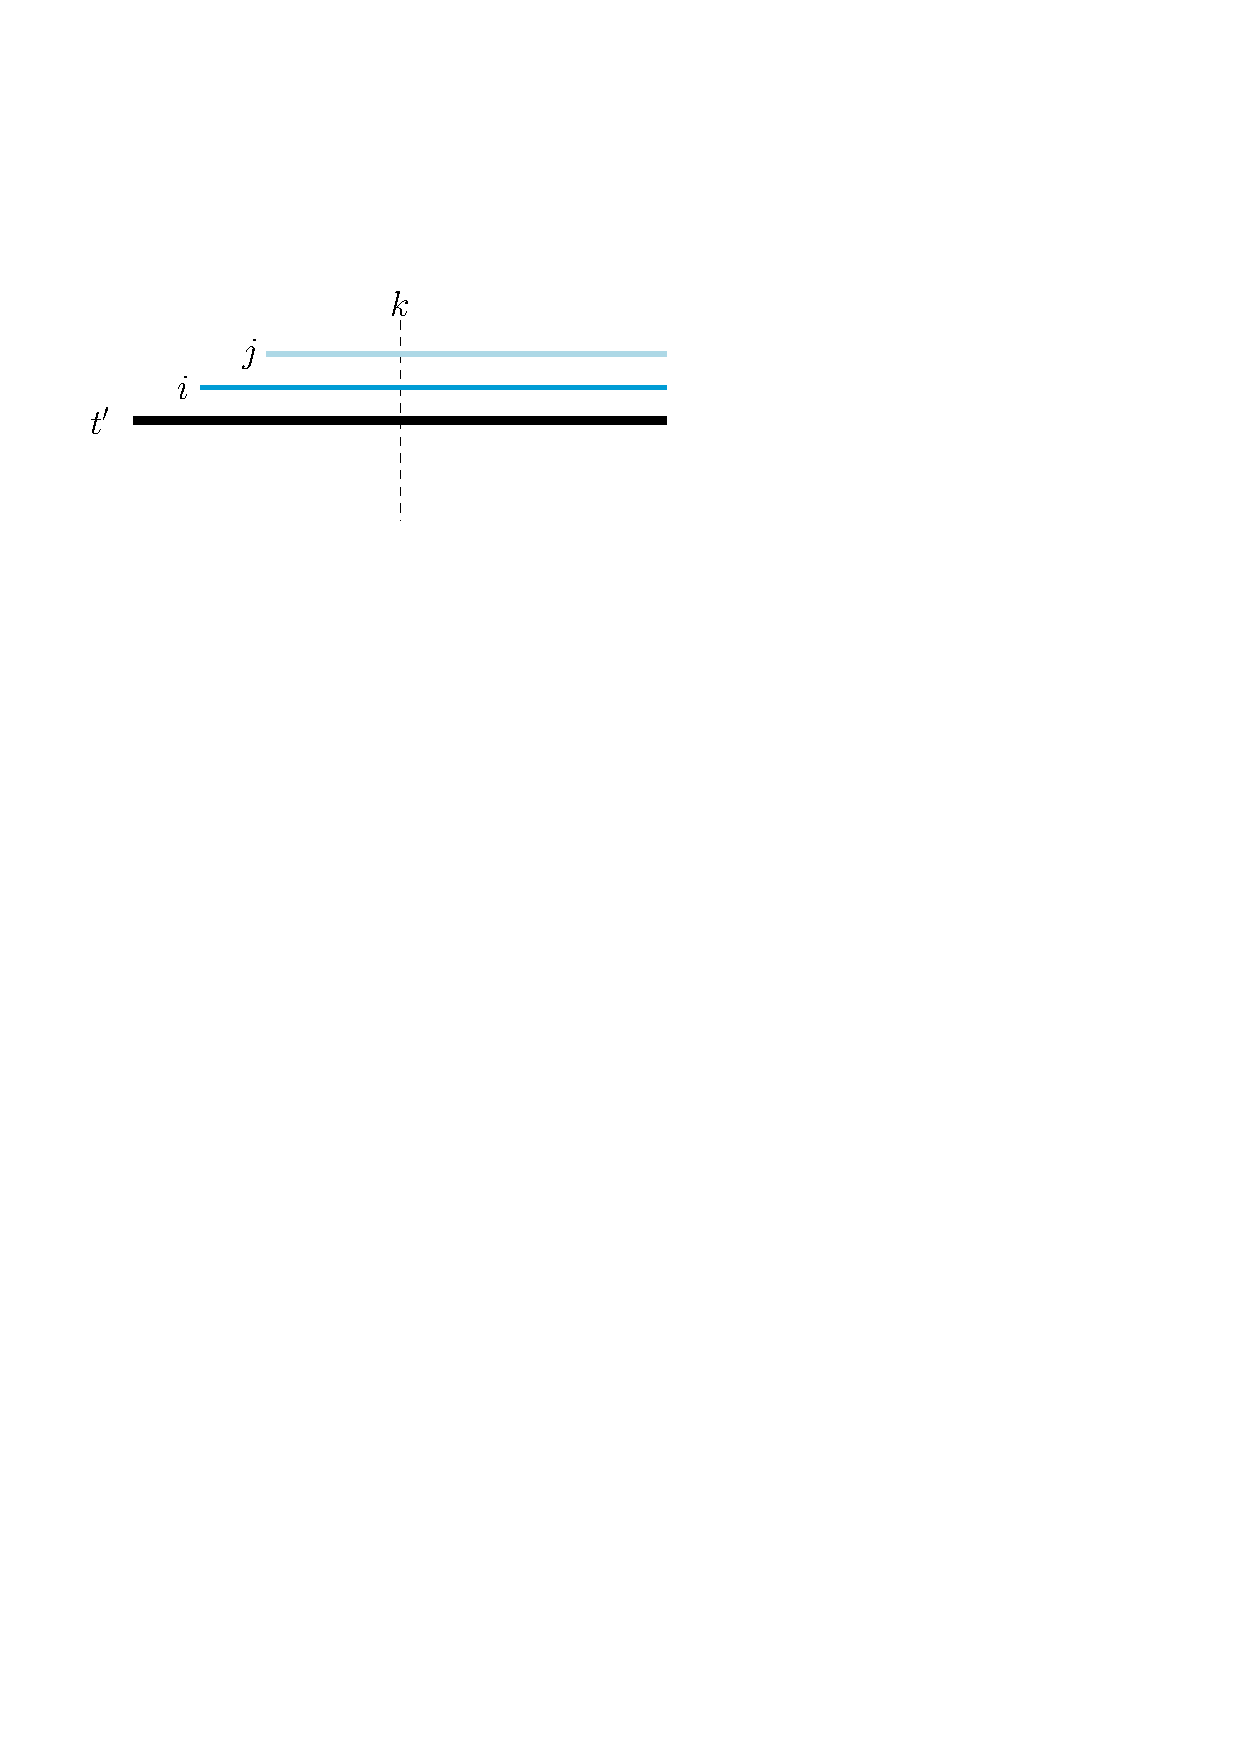
\includegraphics[width=\linewidth]{sa-dc3/case1-t-prime-suffixes.pdf}
    \end{marginfigure}
    More formally, let $k$ be the position such that $\id{pos}[k] \bmod 3 = 1$ but $\id{pos}[k+1] \bmod 3 = 2$. Then, during the comparison of the two suffixes of $t'$ starting at $i$ and $j$, at most $k$ characters are compared. This is because the triple at position $\id{pos}[k]$ will contain the unique \textbf{null terminator} that is lexicographically smaller than any character in the alphabet, thus giving the triple at $\id{pos}[k]$ a \textbf{unique rank}.

    Moreover, each symbol in $t'$ represents the \textbf{rank of a triple} starting at that position in $T$. By assumption, the suffix of $t'$ starting at $i$ is lexicographically smaller than the suffix of $t'$ starting at $j$. Then, there must exists some $c$ such that $t'[i+c] < t'[j+c]$. This implies that the triple starting at position $\id{pos}[j+c]$ that is lexicographically larger than the triple starting at position $\id{pos}[i+c]$ because $t'$ represents the ranks of the triples. The presence of this \textbf{lexicographically larger triple} makes the suffix of the original string at $\id{pos}[i]$ lexicographically smaller than the suffix at $\id{pos}[j]$.
    
    \textbf{Case 2}: Both $i$ and $j$ are in the second half. This case follows from a similar argument as Case 1.

    \begin{marginfigure}
        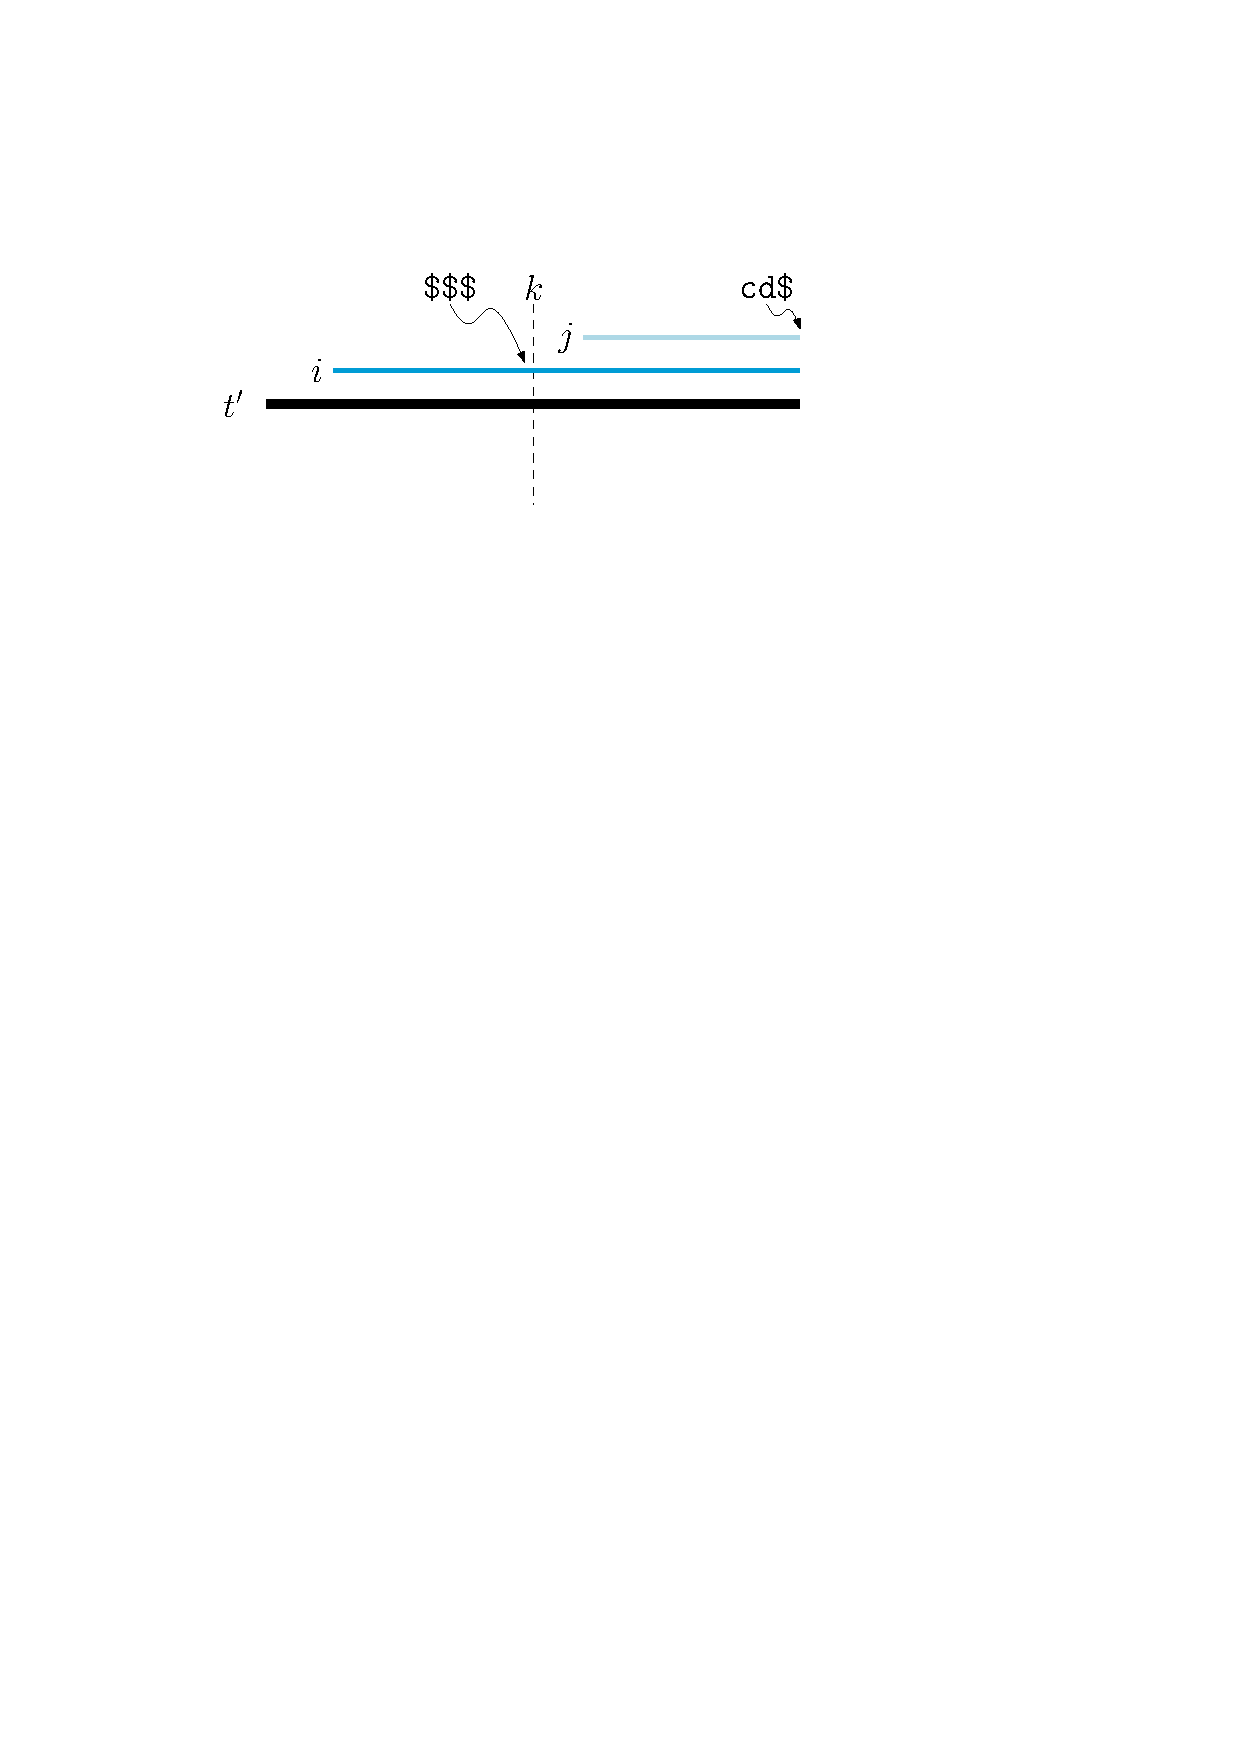
\includegraphics[width=\linewidth]{sa-dc3/case3-t-prime-suffixes.pdf}
    \end{marginfigure}

    \textbf{Case 3}: $i$ is in the first half and $j$ is in the second half. As in the first two cases, the comparison will \textbf{never cross the boundary}. This, again, is due to the distinct null terminator symbol. In particular, the triple starting at $\id{pos}[k]$ (recall that $k$ is the boundary between the two parts) contains at least one more/fewer null terminator symbol compared to the triple at $\id{pos}[|t'|]$. Hence, the triple at $\id{pos}[k]$ will have a \textbf{unique rank}, which helps us \textbf{break the tie} after the comparison at position $k$. We can always determine the lexicographic order of the two suffixes without crossing the boundary.

    Now, going back to $t'$, if we have the suffix of $t'$ starting at $i$ being lexicographically smaller than the suffix of $t'$ starting at $j$, we know that there must be some $c$ such that $t'[i+c] < t'[j+c]$, which implies the rank of some triple at $\id{pos}[i+c]$ is lexicographically smaller than that at $\id{pos}[j+c]$. Since we never cross the boundary when comparing the suffixes of $t'$ starting at $i$ and $j$, we are always comparing the rank of a contiguous and non-overlapping substring of $T$ starting at $\id{pos}[i]$ with the rank of some other contiguous and non-overlapping substring of $T$ at $\id{pos}[j]$ without ever going backward in the comparison (because we don't cross the boundary). Then, it follows that the lexicographic ordering of the ranks in $t'$ implies the ordering in $T$.
    
    \textbf{Case 4}: $i$ is in the second half and $j$ is in the first half. This follows from a similar argument as Case 3.

    In all cases, the implication holds, so the lemma holds.
\end{proof}

One important takeaway from the proof of this lemma is that the null terminator symbol \texttt{\$} is a tie-breaker, giving us unique ranks for triples at the end of the first and second half so that we never cross the boundary between the two halves. This unique rank, in turn, allows us to use the string of ranks to implicitly sort the suffixes in the original string $T$.

Using our previous example with
$$
\begin{array}{ccccccc|cccc}
    \scriptstyle i &  & \scriptstyle 1 & \scriptstyle 2 & \scriptstyle 3 & \scriptstyle 4 & \scriptstyle 5 & \scriptstyle 6 & \scriptstyle 7 & \scriptstyle 8 & \scriptstyle 9 \\
    \id{pos} & = & 1 & 4 & 7 & 10 & 13 &  2 & 5 & 8 & 11 \\
    t_1 \cdot t_2 & = & \texttt{dad} & \texttt{bcd} & \texttt{dad} & \texttt{bcd} & \texttt{\$\$\$} & \texttt{adb} & \texttt{cdd} & \texttt{adb} & \texttt{cd\$} \\
    t' & = & 6 & 3 & 6 & 3 & 1 & 2 & 5 & 2 & 4
\end{array}
$$
we have
$$
\begin{array}{ccccccccccc}
    \text{SA for $t'$} & = & 5 & 8 & 6 & 4 & 2 &  9 & 7 & 3 & 1 \\
    \text{SA$_{12}$ for $T$} & = & 13 & 8 & 2 & 10 & 4 & 11 & 5 & 7 & 1
\end{array}
$$
The $i$th entry in the SA for $T$ is $SA_{12}(T)[i] = \id{pos}[SA(T')[i]]$. Here, $SA_{12}(T)$ refers to the suffix array for the original string $T$ but only considering the suffixes at positions $1$ or $2$ mod $3$.

\subsection{Sorting the Non-Sample Suffixes}

There is an easy way to sort the non-sample suffixes. Those are the suffixes that start at positions $i \bmod 3 = 0$. Again, we begin by considering the triples starting at these positions. Each of such positions is followed by two positions with $i \bmod 3 \neq 0$. Ordering of the triples starting at one and two positions after those with $i \bmod 3 = 0$ have already been determined recursively as discussed in the previous subsection. We can then use the information we know about the sample suffixes to sort the non-sample suffixes in linear time, non-recursively.

To this end, we construct a list $t''$ that contains all characters at positions $i \bmod 3 = 0$ with each character followed by the rank of the suffixes starting at position immediately after $i$ (which can be determined from $SA[t']$ that we have constructed in the previous step).

Slightly more formally, the $i$th element of $t''$ will be
$$
t''[i] = T[3i] \cdot SA_{12}(T)[3i+1]
$$
In our example, $T = \texttt{dadbcddadbcd\$}$ and
$$
\begin{array}{ccccccccccc}
    \scriptstyle i &  & \scriptstyle 1 & \scriptstyle 2 & \scriptstyle 3 & \scriptstyle 4 & \scriptstyle 5 & \scriptstyle 6 & \scriptstyle 7 & \scriptstyle 8 & \scriptstyle 9 \\
    \text{SA for $t'$} & = & 5 & 8 & 6 & 4 & 2 &  9 & 7 & 3 & 1 \\
    \text{SA$_{12}$ for $T$} & = & 13 & 8 & 2 & 10 & 4 & 11 & 5 & 7 & 1
\end{array}
$$
so
$$
\begin{array}{ccccccccccc}
    \text{triple} & = & \texttt{dbc} & \texttt{dda} & \texttt{dbc} & \texttt{d\$\$} \\
    t'' & = & \texttt{d5} & \texttt{d8} & \texttt{d4} & \texttt{d1} \\
    \id{pos} & = & 3 & 6 & 9 & 12
\end{array}
$$
We sort $t''$ using radix sort in $\Theta(n)$ time. For our example, this gives us
$$
\begin{array}{ccccccccccc}
    t'' & = & \texttt{d1} & \texttt{d4} & \texttt{d5} & \texttt{d8} \\
    \id{pos} & = & 12 & 9 & 3 & 6
\end{array}
$$
The corresponding positions in the sorted $t''$ is the suffix array for the suffixes starting at $i \bmod 3 = 0$, so we have $SA_{3}(T)$ as well.

The correctness of this step is trivial from the correctness of radix sort and the fact that the entries in $SA_{12}$ are unique (so there won't be tie).

\subsection{Merging the Two Suffix Arrays}

The final punchline. We will merge $SA_{12}(T)$ and $SA_{3}(T)$ into one suffix array in linear time.

Recall that in the $O(n^2)$ algorithm for constructing a suffix array, the merging is done in $O(n^2)$ time using the naive method. The naive method keeps two pointers to each of the restricted suffix arrays $SA_{12}$ and $SA_{3}$. It then compare the suffixes explicitly in worst-case $O(n)$ time. We do this for all the $O(n)$ pairs of positions, giving us an $O(n^2)$ time algorithm.

\begin{codebox}
    \li $i,j = 1,1$ 
    \li \While $i \leq |SA_{12}(T)|$ and $j \leq |SA_{3}(T)|$  \Do
            \li compare suffixes $T[SA_{12}(T)[i] \ldots]$ and $T[SA_{12}(T)[j] \ldots]$
            \li update $i,j$ accordingly
\end{codebox}

However, with the suffixes arrays $SA_{12}$ and $SA_3$, we can actually do the comparison in constant time. For each arbitrary pair of positions $i,j$, we only need at most $3$ explicit character comparisons before we reach a position $i',j'$ such that $i' = j' \mod 3$, at which point the lexicographic order of the two suffixes can be determined using an $O(1)$ \textbf{lookup} in the appropriate restricted suffix array.

For a more detailed procedure for merging, consider the following cases:

\textbf{Case 1}: Compare two suffixes starting at $i$ and $j$ where $i \bmod 3 = 2$ and $j \bmod 3 = 0$. If the encounter a character such that $T[i] \neq T[j]$, then we are done. Otherwise, continue comparing $T[i]$ with $T[j]$ and updating $i$ and $j$. After at most 2 comparisons, $i \bmod 3 = 1$ and $j \bmod 3 = 2$. We can determine the ordering of the two suffixes by comparing the locations of $i$ and $j$ in $SA_{12}$ in $O(1)$ time.

\textbf{Case 2}: Compare two suffixes starting at $i$ and $j$ where $i \bmod 3 = 1$ and $j \bmod 3 = 0$. If we encounter a character such that $T[i] \neq T[j]$, then we are done. Otherwise, the problem reduces to Case 1, and we can determine the lexicographic ordering of the suffixes starting at $i$ and $j$ with at most $3$ explicit comparisons.

\textbf{Case 3}: $i = j \mod 3$. This case is trivial through a constant-time lookup in $SA_{12}$ if $i \bmod 3 = j \bmod 3 \neq 0$ or in $SA_{3}$ if $i \bmod 3 = j \bmod 3 = 0$.

In all three cases, we can determine the lexicographic ordering of the two suffixes within $O(1)$ comparisons. We repeat this for all $|T|$ positions, giving us an $O(n)$ time algorithm for merging.

\subsection{Wrapping It Up}

And here we have it, the linear-time algorithm for constructing a suffix array. At first glance, it appears to be quite a sophisticated algorithm, but the ideas behind it are actually quite fundamental. It based on the same divide-and-conquer approach that previous $O(n^2)$ and $O(n \log n)$ time algorithms have used, but with a few ingenious improvements that allow us to do the merging in $O(n)$ time. Note that the linear-time merging is not possible if we divide the suffixes up into positions $0$ or $1$ mod $2$ since we are not guaranteed to be at a position $i=j \mod 2$ after just a constant number of comparisons.

As we mentioned at the beginning, this algorithm is due to Karkkainen and Sanders. It is often referred to as the \textit{\textbf{Karkkainen-Sanders (KS) algorithm}} or the \textit{\textbf{DC3 algorithm}} since it is a divide-and-conquer algorithm that divides the positions based on their values modulo 3.

To wrap this section up, let us prove that the KS algorithm indeed runs in linear time.

\begin{theorem}
    The suffix array for text $T$ of length $n$ can be computed in time $O(n)$.
\end{theorem}

\begin{proof}
    We use the Karkkainen-Sanders' algorithm. The correctness of the algorithm is argued as we introduce the algorithm. Now, we consider the runtime of the algorithm.

    Sorting of the triples takes $O(n)$ time using radix sort, and so does the computation of the SA for the non-sample suffixes at position $i \bmod 3 = 0$. At each level of the recursion, the suffix array that we recursively construct is of size $\lceil 2/3n \rceil$. Finally, merging takes $O(n)$ time. Hence, the overall runtime is given by the recurrence
    $$
    \begin{aligned}
        T(n) &= T(\lceil 2/3n \rceil) + 3O(n) \\
        &= T(\lceil 2/3n \rceil) + O(n) \\
        &\leq n \sum_{i=0}^\infty \left( \frac{2}{3} \right)^i \\
        &\in O(n) 
    \end{aligned}
    $$
    The same recurrence can also be solved using the Master's theorem.
\end{proof}